\documentclass[A4paper,11pt]{article}

\usepackage{latexsym}
\usepackage{epsfig}
\usepackage{verbatim}
\usepackage{shadow}
\usepackage{amssymb}
\usepackage{amsmath}
\usepackage{graphicx}
\usepackage{color}
\usepackage{bm}
\usepackage{fancyhdr}

\addtolength{\textwidth}{4cm}
\addtolength{\textheight}{6.9cm}
\addtolength{\oddsidemargin}{-2cm}
\addtolength{\topmargin}{-4.9cm}

\newtheorem{theorem}{\sc Theorem}[section]
\newtheorem{lemma}[theorem]{\sc Lemma}
\newtheorem{corollary}[theorem]{\sc Corollary}
\newtheorem{fact}[theorem]{\sc Fact}
\newtheorem{remark}[theorem]{\sc Remark}

\author{
	{\sc Guangyu Dong} \\
	\texttt{gdong2@illinois.edu}
	\and
	{\sc Randolph Hill} \\
	\texttt{rwhill2@illinois.edu}
	\and
	{\sc Vasileios Livanos} \\
	\texttt{livanos3@illinois.edu}
}

\title{
Resource-Constrained Social Networks under Prospect Theory
}

\date{}

\begin{document} \maketitle

\par Consider $n$ agents that interact with each other in a social network. Each agent $i$ has a specific set of other agents
that they interact with, which is called the \textit{neighborhood} of $i$ and is denoted by $\mathcal{N}_i$. In this network,
each agent has a set of strategies available to them. Specifically, agent $i$ proposes an \textit{interaction frequency}
$f_{ij} \in \mathbb{R}$ to every agent $j \in \mathcal{N}_i$. Similarly, each agent $j$ proposes an
interaction frequency $f_{ji}$ to $i$. The frequency that they end up interacting at is simply the minimum of the two
proposals. However, in real social networks, the agents have different preferences for who to interact with. To capture this
in our model, we assign $w_{ij}$ to be the \textit{weight} $i$ places on $j$, or similarly how much $i$ values the interaction
with $j$. Further motivated by real social networks, we assign all agents a uniform ``budget" of interaction frequency $\beta$
that they cannot exceed.

\par In our model we deviate from standard practices in algorithmic game theory and instead of considering that agents act
in accordance with the predictions of the expected utility theory, we consider the case where the behavior of the network's
agents is better captured by \textit{prospect theory}. Prospect theory, introduced by Kahneman and Tversky \cite{KT}, states
that people make decisions based on the potential value of losses and gains rather than the final outcome, and that people
evaluate these losses and gains using certain heuristics. This model attempts to depict real-life scenarios, where the agents
sometimes act irrationally rather than making the optimal decisions for them. Therefore, we consider utility functions that
capture the observation of prospect theory that in real-life situations people are \textit{loss-averse}; in mathematical terms,
if $u_i(x)$ is the utility of player $i$ with $x$ being the strategy profile, then $- u_i(-x) > u(x)$. In other words, utility
functions studied by prospect theory are similar to the one in Figure \ref{fig:prospect-util}, with the curve for losses being
``steeper" than the curve for gains.

\begin{figure}[h!]
  \centering
  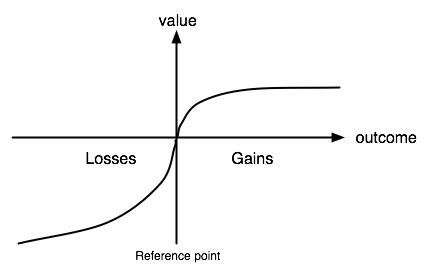
\includegraphics[width=.30\linewidth]{./Valuefun.jpg}
  \caption{An agent's utility function as described by prospect theory}
  \label{fig:prospect-util}
\end{figure}

\par It is clear that our approach is motivated by real-life social networks therefore an analysis would not be complete
if it remained in a theoretical level. To this end, we gather data from real online social networks such as Stack Overflow. We
will collect and evaluate how an agent's post frequency changes in this type of network in relation to the ``up-votes" the agent
receives. We evaluate this behavior over the entire network and compare the expected convergence over all users.  This will be
evaluated by modeling the network with respect to expected utility theory and then comparing the convergence properties when
modeled with prospect theory preferences. This real world model will help us understand whether the observations from real social
networks are similar to the predictions of our model.

\label{Bibliography}

\lhead{\emph{Bibliography}}

\bibliographystyle{abbrv}

\bibliography{one-pager} % The references (bibliography) information are stored in the file named "Bibliography.bib"

\end{document}
